\documentclass[12pt, twoside]{article}
\usepackage[letterpaper, margin=1in, headsep=0.5in]{geometry}
\usepackage[english]{babel}
\usepackage[utf8]{inputenc}
\usepackage{amsmath}
\usepackage{amsfonts}
\usepackage{amssymb}
\usepackage{tikz}
%\usetikzlibrary{quotes, angles}

\usepackage{graphicx}
\usepackage{enumitem}
\usepackage{multicol}

\usepackage{fancyhdr}
\pagestyle{fancy}
\fancyhf{}
\renewcommand{\headrulewidth}{0pt} % disable the underline of the header

\fancyhead[RE]{\thepage}
\fancyhead[RO]{\thepage \\ Name: \hspace{3cm}}
\fancyhead[L]{BECA / Dr. Huson / 10th Grade Geometry\\* Unit 9 Transformations\\29 March 2019}

\begin{document}
\subsubsection*{9-4 Homework: Applying Algebra to Geometric Situations}
  \begin{enumerate}

  \item The line $l$ has the equation $y=-\frac{2}{3}x+5$. To each line below, circle whether $l$ is parallel, perpendicular, or neither.
    \begin{enumerate}
      \item parallel \quad perpendicular \quad neither \qquad $y=-\frac{2}{3}x-2$
      \vspace{0.5cm}
      \item parallel \quad perpendicular \quad neither \qquad $y=\frac{3}{2}x+9$
      \vspace{0.5cm}
      \item parallel \quad perpendicular \quad neither \qquad $2x-3y=12$
      \vspace{2cm}
      \item parallel \quad perpendicular \quad neither \qquad $3x+2y=-4$
      \vspace{2.5cm}
    \end{enumerate}

    \item What is the equation of a line through $A(4,1)$ and parallel to the line $y=\frac{1}{2}x-5$? (hint: use the point-slope formula, $y-y_A=m (x-x_A)$) \vspace{2cm}

  \item Simplify each expression. (Leave it in radical form if necessary, not a decimal.)
    \begin{enumerate}
      \begin{multicols}{2}
      \item   $\sqrt{20}$ \vspace{1.5cm}
      \item   $\sqrt{\frac{4}{25}}$ \vspace{1.5cm}
      \end{multicols}
    \end{enumerate}
    \vspace{2cm}


  \item Write down the center and radius of each circle.
    \begin{enumerate}
      \begin{multicols}{2}
      \item   $(x-1)^2+(y+4)^2=49$ \vspace{2cm}
      \item   $(x+6)^2+(y-1)^2=4$
      \item   $(x-9)^2+(y+1)^2=7$ \vspace{2cm}
      \item   $(x-1)^2+(y+4)^2=16$
      \end{multicols}
    \end{enumerate}  \vspace{2cm}

\newpage

 \item Given $\triangle ABP$ and $\triangle JKP$ as shown below. $\overline{AB} \parallel \overline{JK}$. $AP=6.3$, $JP=12.6$, and $JK=17$. Find $AB$.
 \begin{center}
   \begin{tikzpicture}[scale=1.4]
       \draw [thick]
         (0.25,-1)node[right]{$B$}--
         (-0.5,2)node[left]{$K$}--
         (4,0)node[right]{$J$}--
         (0,0)node[above right]{$P$}--
         (-2,0)node[left]{$A$}--cycle;
     \end{tikzpicture}
     \end{center}

 \vspace{3cm}

   \item The vertices of $\triangle JKL$ have the coordinates $J(-4,3)$, $K(-1,-1)$, and $L(-2,4)$, as shown below. \\[0.25cm]
   Apply a translation of $(x,y) \rightarrow (x+5, y+1)$ to $\triangle JKL$ and then reflect the image across the $x$-axis. Draw both images $\triangle J'K'L'$ and $\triangle J''K''L''$ on the set of axes below, labeling the vertices.
   \begin{center}
     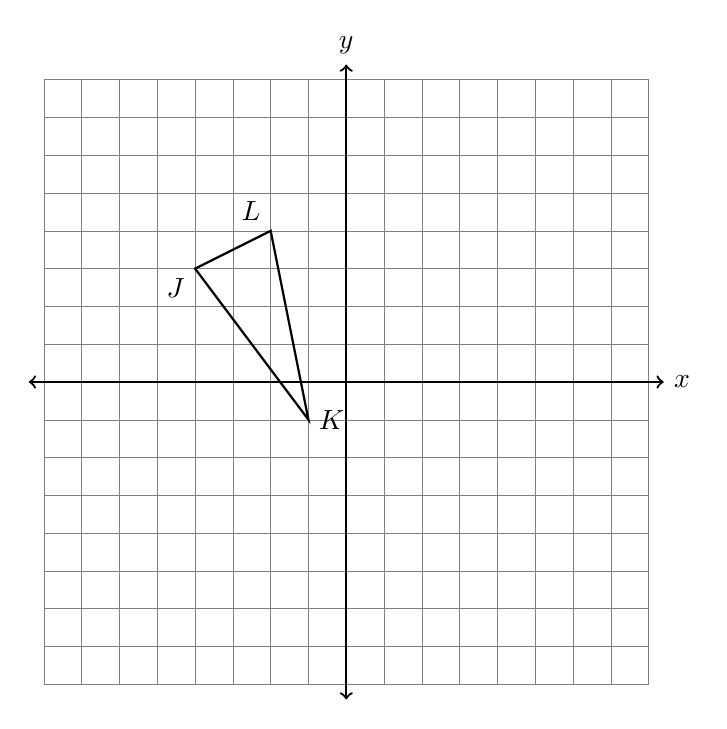
\begin{tikzpicture}[scale=.48]
       \draw [help lines] (-8,-8) grid (8,8);
       \draw [thick, <->] (-8.4,0) -- (8.4,0) node [right] {$x$};
       \draw [thick, <->] (0,-8.4)--(0,8.4) node [above] {$y$};

       \draw [thick]
       (-4,3) node[below left] {$J$}--
       (-1,-1) node[right] {$K$}--
       (-2,4) node[above left] {$L$}--
       cycle;
     \end{tikzpicture}
   \end{center}

\newpage

  \item A translation maps $P(-1,5) \rightarrow P'(3,-2)$. What is the image of $Q(3,4)$ under the same translation?  \vspace{3cm}

  \item As shown below, what is the translation that maps the point $R(-3,2)$ onto the point $S(6, 5)$?
    \begin{center} %4 quadrant regents grid
      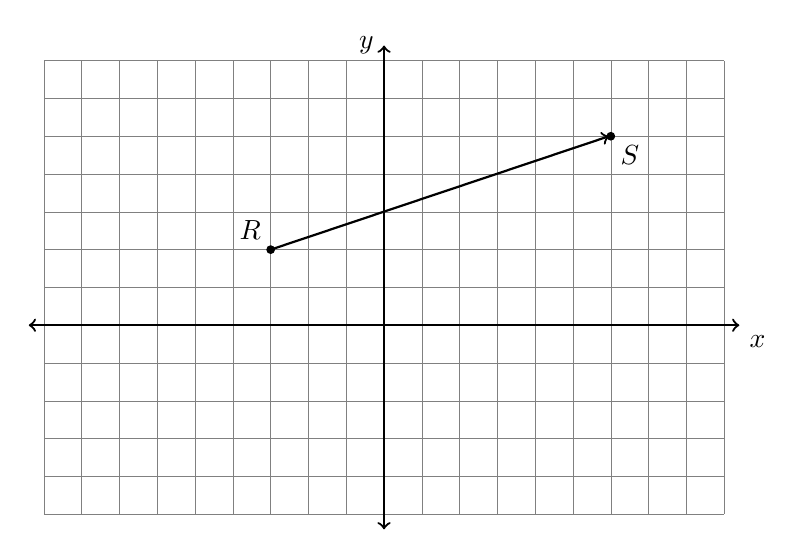
\begin{tikzpicture}[scale=.48]
        \draw [help lines] (-9,-5) grid (9,7);
        \draw [thick, <->] (-9.4,0) -- (9.4,0) node [below right] {$x$};
        \draw [thick, <->] (0,-5.4)--(0,7.4) node [left] {$y$};
        \draw [thick, ->] (-3,2)--(5.95, 5);
        \draw [fill] (-3,2) circle [radius=0.1] node[above left] {$R$};
        \draw [fill] (6, 5) circle [radius=0.1] node[below right] {$S$};
      \end{tikzpicture}
    \end{center}
    If two thirds of that translation was performed, what coordinates would $R$ be mapped to? \vspace{2cm}

  \item Given $A(-3,4)$ and $B(1,-4)$, find the length of $\overline{AB}$. Leave the result in simplified radical form (not a decimal).
      \vspace{4cm}

\newpage

  \item $\triangle ABC$ undergoes two tranformations mapping it onto $\triangle A''B''C''$, as shown below. Specify the two tranformations in order. Complete a table showing the coordinates of the translated points.\\[2cm]
   \hspace{1cm} $A(-6,-1) \rightarrow$\\[1cm]
   \hspace{1cm} $B(-8,2) \rightarrow$\\[1cm]
   \hspace{1cm} $C(-1,3) \rightarrow$

    \vspace{1.5cm}

      \begin{center} %4 quadrant regents grid w T-Chart
      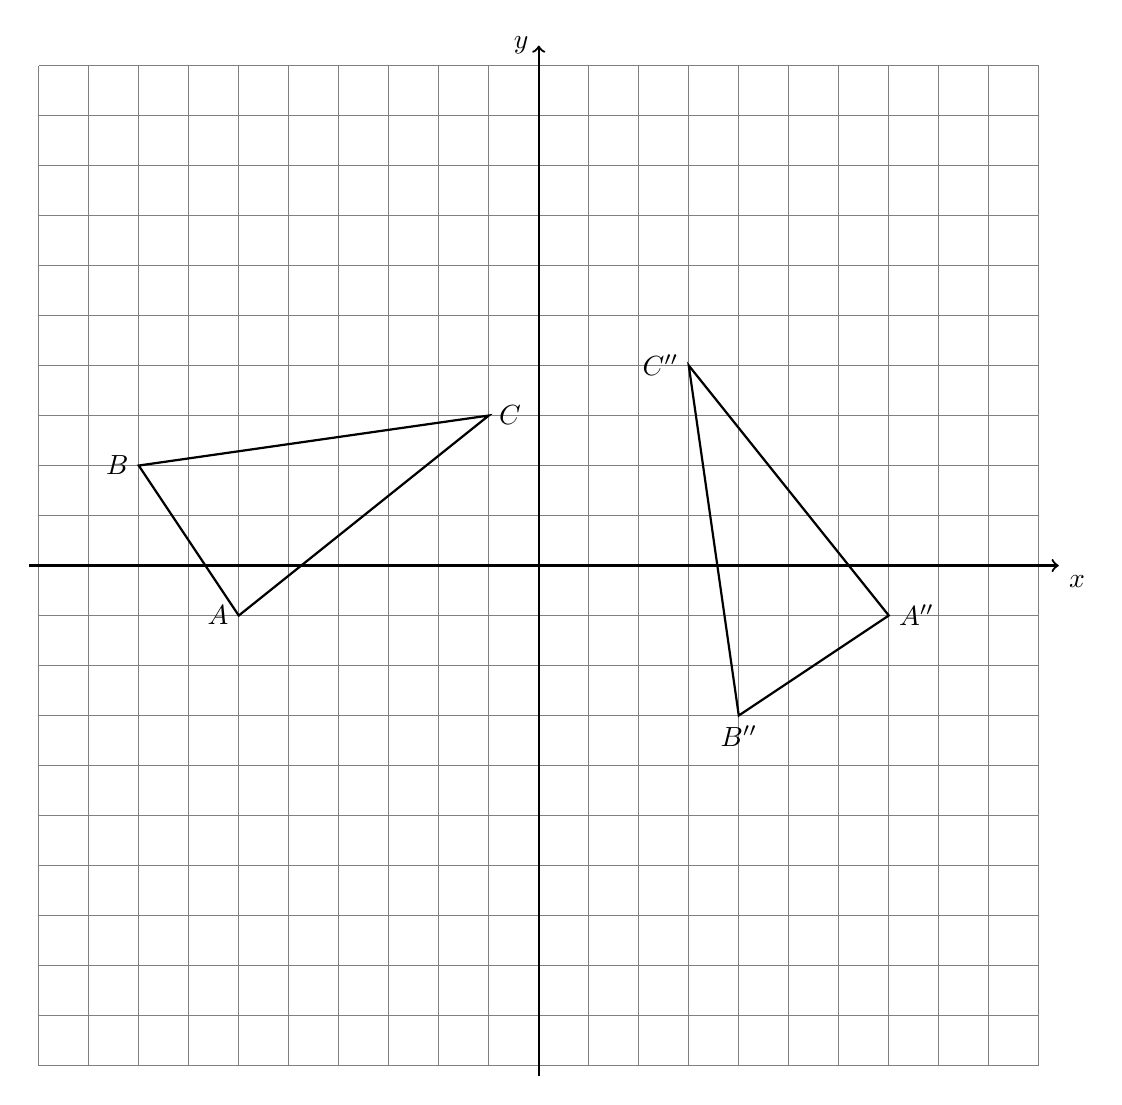
\begin{tikzpicture}[scale=.635]
        \draw [help lines] (-10,-10) grid (10,10);
        \draw [thick, ->] (-10.2,0) -- (10.4,0) node [below right] {$x$};
        \draw [thick, ->] (0,-10.2)--(0,10.4) node [left] {$y$};
        \draw [thick] (-6,-1)node[left]{$A$}--
          (-8,2)node[left]{$B$}--
          (-1,3)node[right]{$C$}--cycle;
        \draw [thick] (7,-1)node[right]{$A''$}--
          (4,-3)node[below]{$B''$}--
          (3,4)node[left]{$C''$}--cycle;
      \end{tikzpicture}
      \end{center}

  \end{enumerate}

  \end{document}
